\documentclass[border=4pt]{standalone}
\usepackage{fontspec}
\usepackage{amsmath}
\usepackage{unicode-math}
\setmainfont{Latin Modern Roman}
\setmathfont{Latin Modern Math}
\usepackage{pgfplots}
\usepackage{pgfplotstable}
\pgfplotsset{compat=1.18}
\usepackage{tkz-euclide}
\usetikzlibrary{arrows.meta,calc,angles,quotes,patterns,3d,backgrounds}
\definecolor{ink}{HTML}{123428}
\definecolor{asy}{HTML}{475569}
\definecolor{mint}{HTML}{86e0bd}
\tikzset{asym/.style={asy, line width=0.9pt, dash pattern=on 5pt off 3.5pt},
         guide/.style={gray!70, line width=0.6pt, densely dotted},
         dot/.style={circle, inner sep=0pt, minimum size=5pt, draw=white, line width=0.5pt},
         odot/.style={circle, inner sep=0pt, minimum size=5.5pt, fill=white, line width=1pt},
         lab/.style={font=\footnotesize, inner sep=1.5pt, text=ink}}
\begin{document}
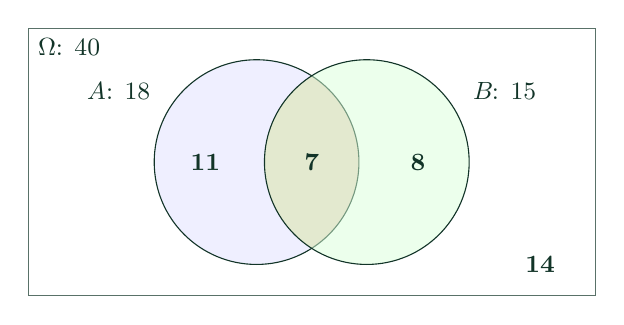
\begin{tikzpicture}[font=\small, every node/.style={text=ink}]
\draw[ink!70] (-3.6,-1.7) rectangle (3.6,1.7); \node[anchor=north west] at (-3.6,1.7) {$\Omega$: 40};
\begin{scope} \clip (-0.7,0) circle (1.3); \fill[orange!45] (0.7,0) circle (1.3); \end{scope}
\draw[ink, fill=blue!12, fill opacity=0.5] (-0.7,0) circle (1.3); \draw[ink, fill=green!15, fill opacity=0.5] (0.7,0) circle (1.3);
\node at (-1.35,0) {\textbf{11}}; \node at (0,0) {\textbf{7}}; \node at (1.35,0) {\textbf{8}}; \node at (2.9,-1.3) {\textbf{14}};
\node at (-2.45,0.9) {$A$: 18}; \node at (2.45,0.9) {$B$: 15};
\end{tikzpicture}
\end{document}
